\chapter{\todo{Skew Octupolar Fields}}
\label{chapter:skew_octupole_fields}
\thumbforchapter{}
\chaptertoc{}
%\newpage


%=============================
%        Introduction
%=============================
\section{\review{Introduction}}

The skew octupolar fields in the LHC have previously been identified as significant contributors to 
limits in forced dynamic aperture, being the dynamic aperture when kicking the beam with the
AC-Dipole~\cite{carlier_nonlinear_2020}. Skew octupolar correctors are positioned around the
ATLAS and CMS detectors, in Interaction Regions 1 and 5. Those correctors are \textit{common
aperture} magnets ; both beams are affected by the created magnetic fields. Unfortunately, one of
these four correctors, located to the left of ATLAS, is not functioning. As a result, although
corrections can be calculated, they will not effectively minimize the skew octupolar RDTs of
interest, $f_{1012,y}$ and $f_{1210,x}$. 
The associated resonances and frequency lines of these RDTs are shown in
\cref{tab:skew_octupolar:resonances_rdts}.

\begin{table}[!htb]
    \centering
    \begin{tabular}{lccc}
      \toprule
      RDT         & Resonance                &  H-line                    & V-line         \\
      \midrule
      $f_{1012}$  & $\phantom{-}1Q_x - 1Q_y$ &  $\phantom{2Q_x-\ \,}1Q_y$ & $-1Q_x + 2Q_y$ \\
      $f_{1210}$  & $-1Q_x + 1Q_y$           &  $2Q_x - 1Q_y$             & $\phantom{-}1Q_x\phantom{+2Q_y\ \,}$    \\
      \bottomrule
    \end{tabular}
    \caption{Skew octupolar RDTs of interest, their associated resonances and the frequency spectrum
    lines they contribute to.}
    \label{tab:skew_octupolar:resonances_rdts}
\end{table}

First corrections of skew octupolar RDTs were performed in 2018 at top
energy~\cite{carlier_nonlinear_2020}. A different approach for the same corrections is presented in
this chapter.
Measurements were also performed at injection energy with the prospect of corrections. However, it
was observed that Landau octupoles were strongly contributing to the RDTs of interest.


%=============================
%         Top Energy
%=============================
\section{\todo{Corrections at Top Energy}}

The very first skew octupolar RDT corrections in the LHC were made in 2018 during
Run~2~\cite{carlier_nonlinear_2020}. These corrections were computed by matching the RDT level of
the measurements in simulation. This is possible and remains viable as only three correctors are
used and values can be manually adjusted.
In this section, a different approach is taken, based on response matrices. This type of correction
is explained in details in \cref{correction_principle:response_matrix}. The real and imaginary 
responses of the RDTs for each corrector at an arbitrary strength are simulated through tracking.
These responses are collected into a matrix, allowing the determination of the required strengths to
match the RDT level observed in the measurements. Inverting these values result in a correction.


%-----------------------------
%     Correctors Response
%-----------------------------
\subsection{\review{Correctors}}

To create a response matrix, simulations were conducted with the tunes and AC-Dipole deltas set to
those used for measurements. The natural tunes are $Q_x = 0.285$ and $Q_y = 0.292$ while the driven
tunes are $\Delta Q_x = -0.008$ and $\Delta Q_y = 0.01$. Each corrector is then powered
individually for each tracking simulation. For this type of simulation, field errors are not
necessary, as only the RDT shift caused by the corrector relative to the baseline is needed.
\Cref{fig:skew_octupolar:response_correctors} shows the real part of the resulting RDTs from these
simulations for Beam 1. Beam 2 shows a similar level of response for these correctors.

\begin{figure}[!htb]
    \centering
    \begin{subfigure}{0.8\textwidth}
        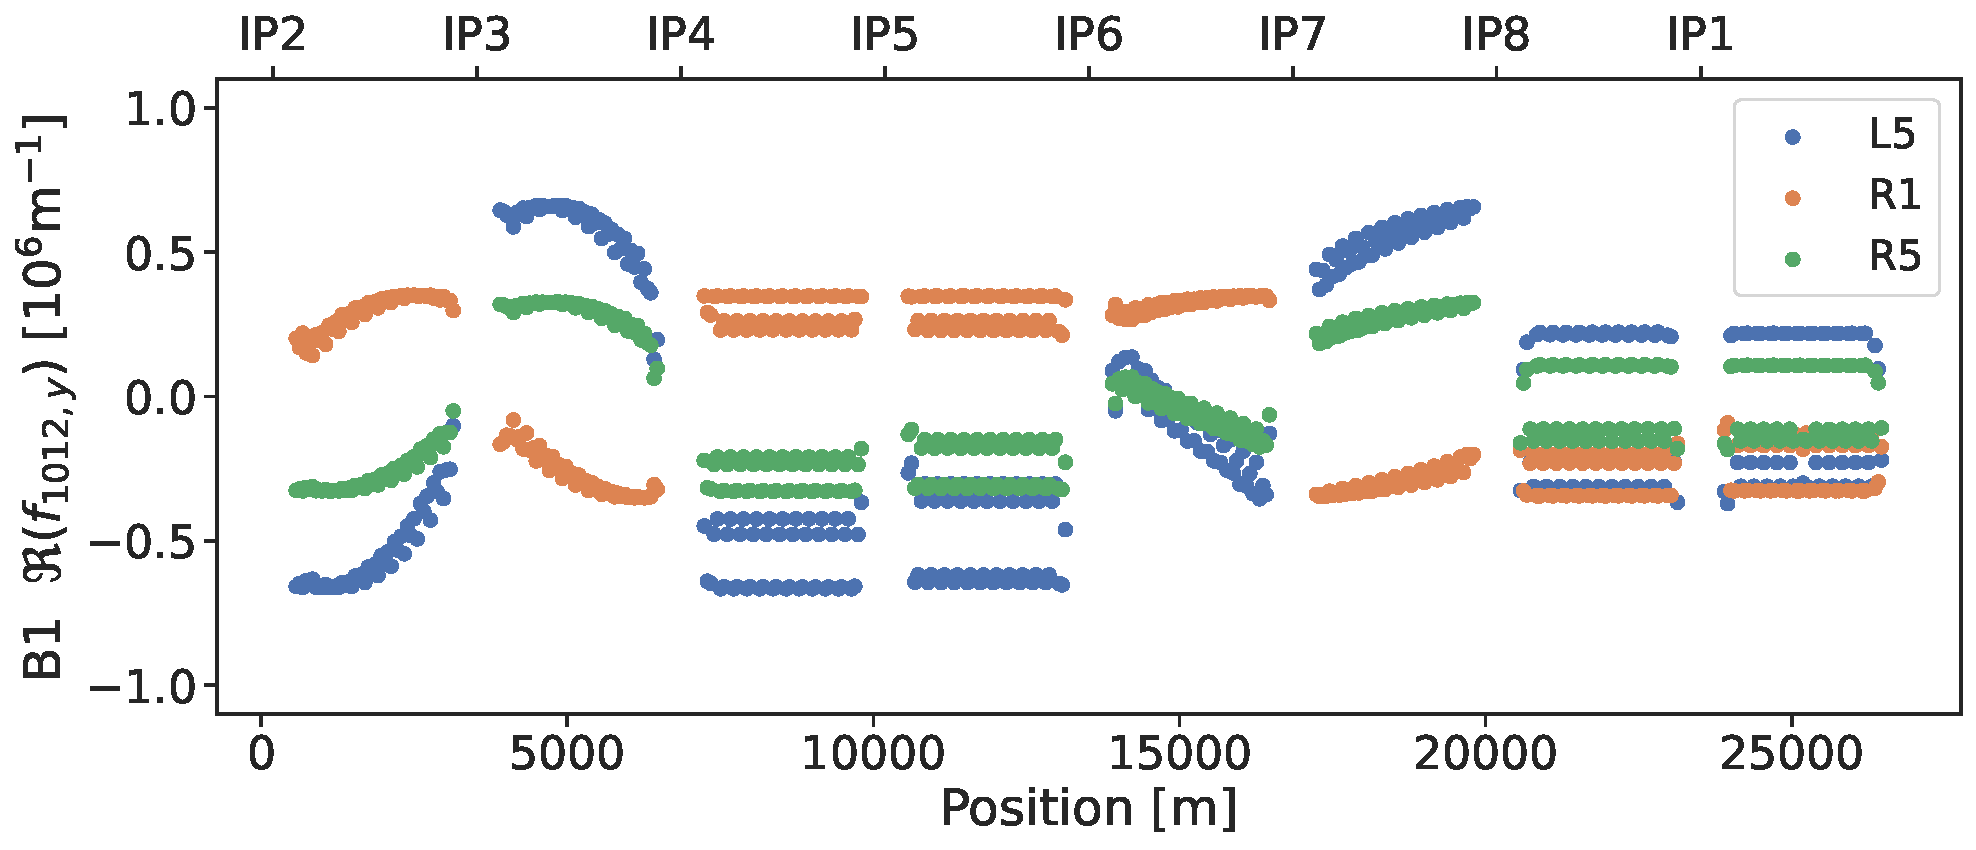
\includegraphics[width=\textwidth]{./images/f1012_b1_correctors.pdf}
        \caption{$f_{1012,y}$}
    \end{subfigure}
    \par\bigskip 
    \begin{subfigure}{0.8\textwidth}
        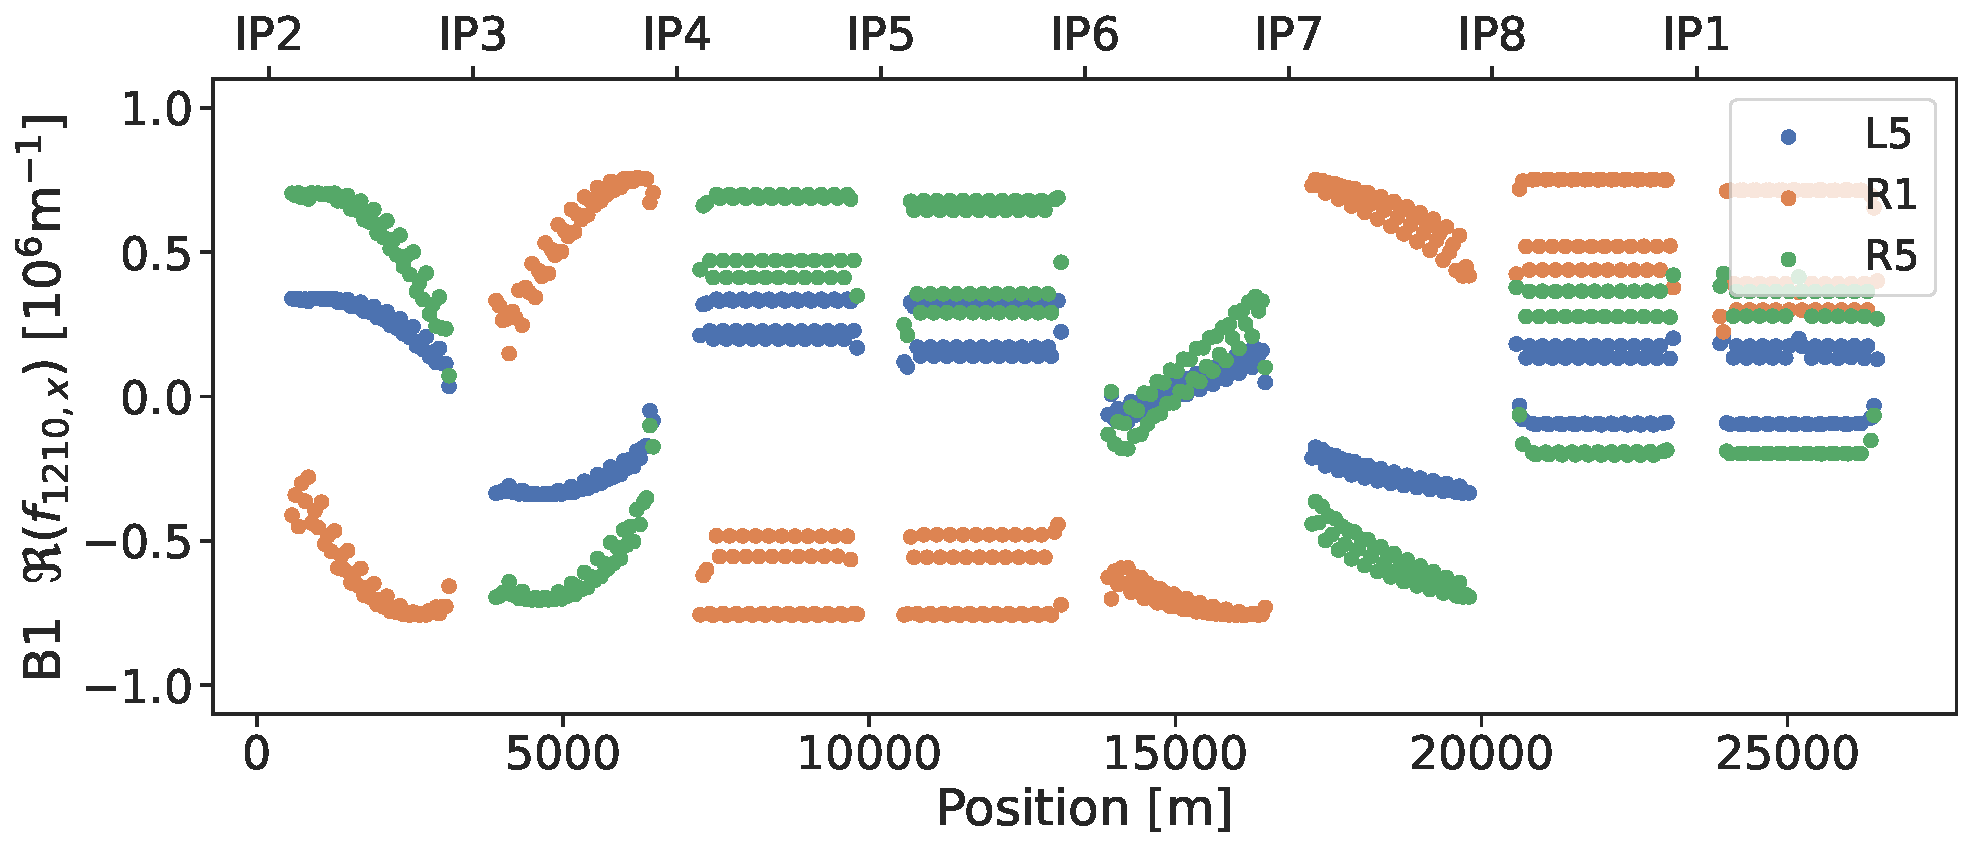
\includegraphics[width=\textwidth]{./images/f1210_b1_correctors.pdf}
        \caption{$f_{1210,x}$}
    \end{subfigure}
    \caption{Simulation of the RDT response of the skew octupolar correctors at top energy for Beam
    1. Each corrector is powered at $J_4 = 1 [\text{m}^{-4}]$.}
    \label{fig:skew_octupolar:response_correctors}
\end{figure}

It can already be seen that the L5 and R5 correctors show a similar trend along the ring, with L5
showing a stronger response for the same strength, while the R1 corrector follows the opposite
trend. A polar plot at a given BPM can illustrate that trend, and be used to get an intuition of the
effect of the correctors to manually compute corrections.
\Cref{fig:skew_octupolar:response_correctors_polar} shows the orthogonality of the correctors for
both beams and RDTs. L5 being stronger than R5 while having the same angle indicates that only one
of them is needed for corrections. 

\begin{figure}[!htb]
    \centering
    \begin{subfigure}{0.8\textwidth}
        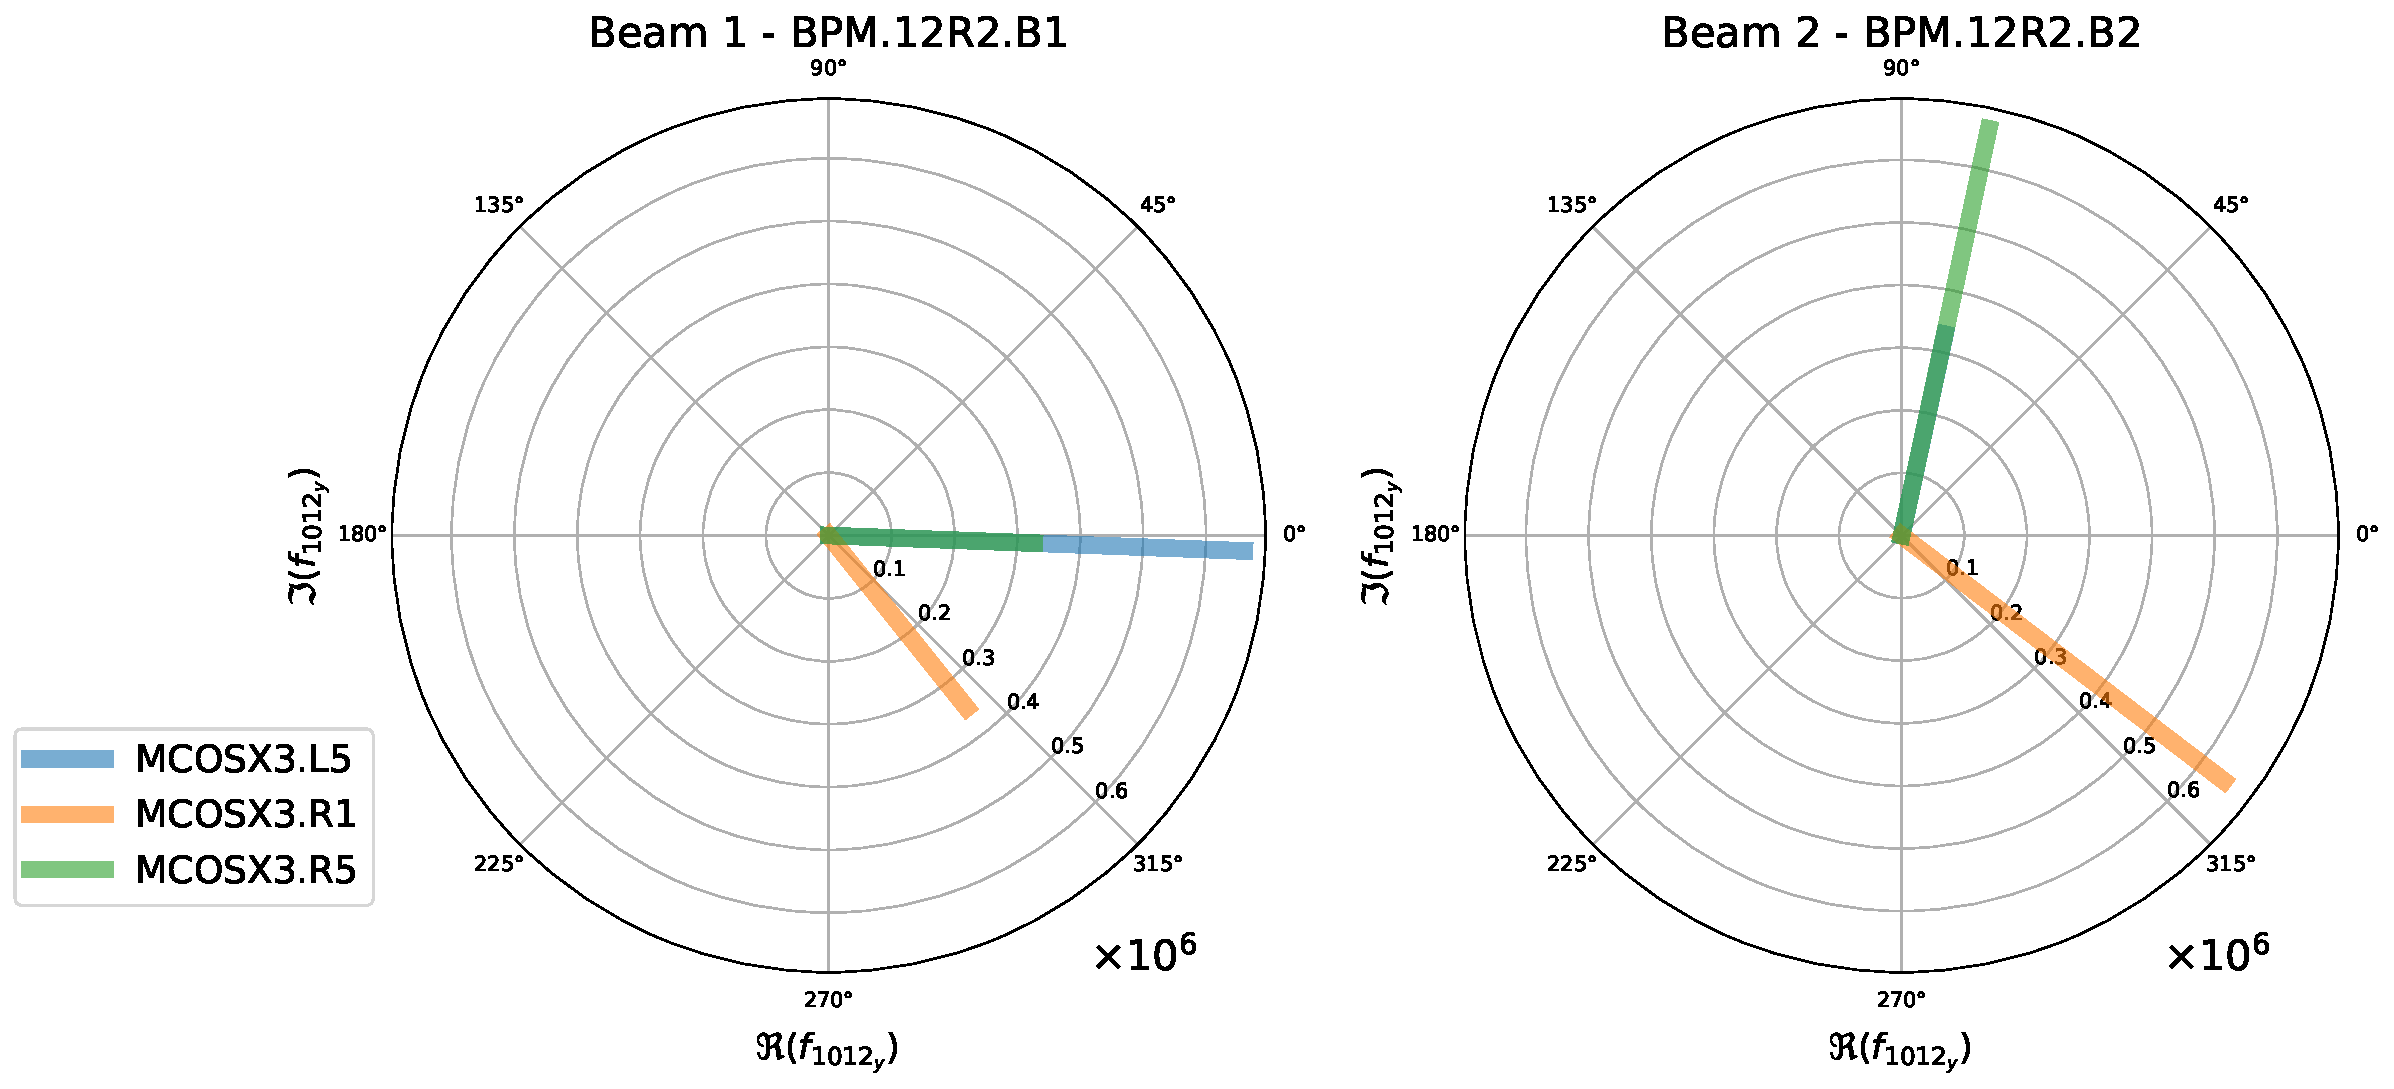
\includegraphics[width=\textwidth]{./images/orthogonal_a4_inj_f1012_y.pdf}
        \caption{$f_{1012,y}$}
    \end{subfigure}
    \par\bigskip 
    \begin{subfigure}{0.8\textwidth}
        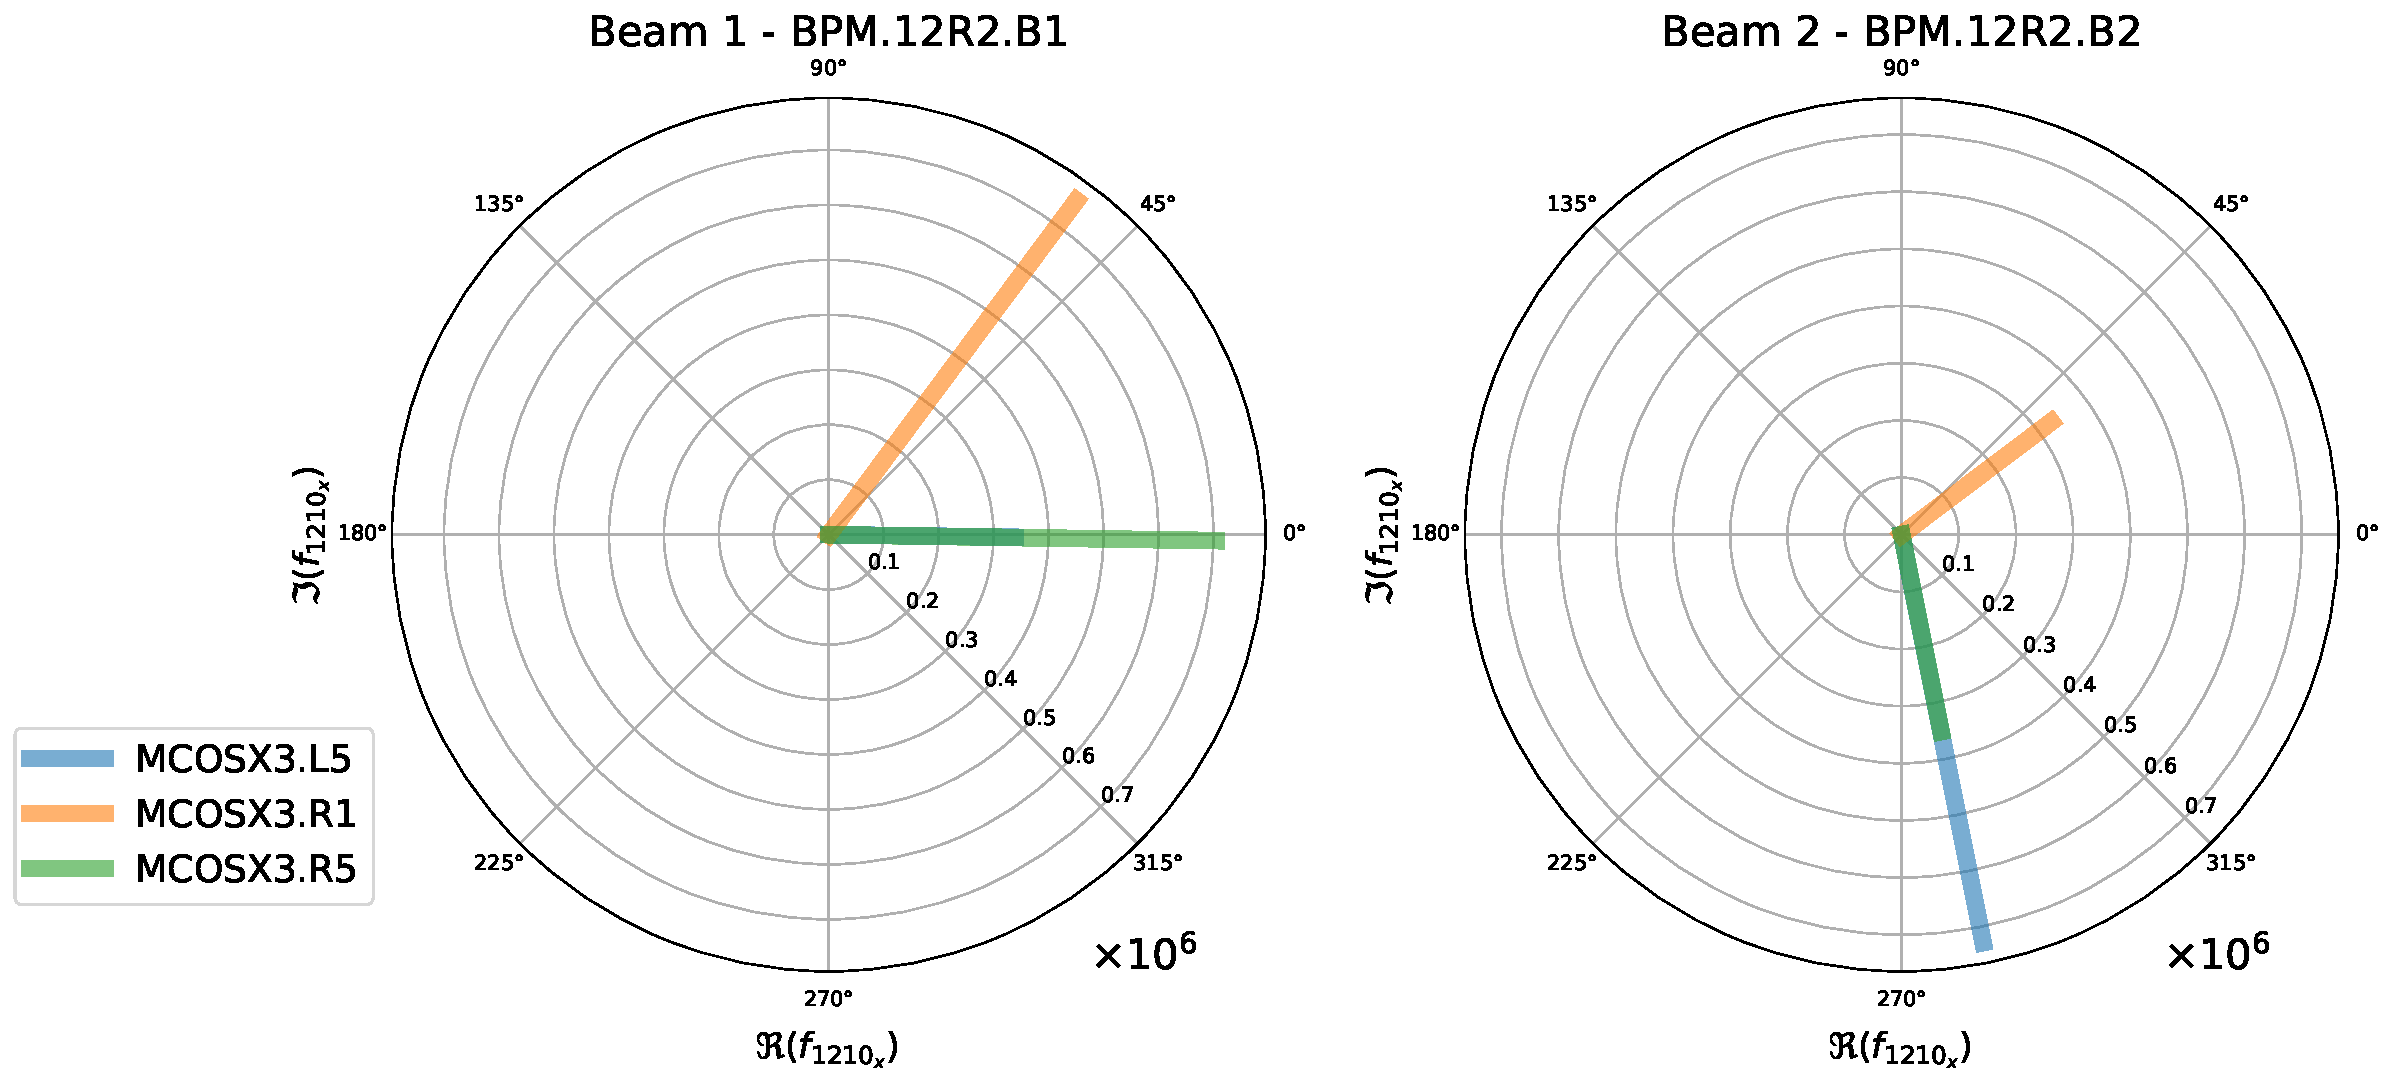
\includegraphics[width=\textwidth]{./images/orthogonal_a4_inj_f1210_x.pdf}
        \caption{$f_{1210,x}$}
    \end{subfigure}
    \caption{Simulated RDTs response of the available skew octupolar correctors at top energy.  Each
    corrector is powered at $J_4 = 1 [\text{m}^{-4}]$. The orthogonality of R1 and L5/R5 allows to
    independently control the real and imaginary parts.}
    \label{fig:skew_octupolar:response_correctors_polar}
\end{figure}



%-----------------------------
%         Correction
%-----------------------------
\subsection{\todo{Measurements and Corrections}}

\todo{impact?}

Initial measurements of the machine at top energy ($\beta^*=30$cm) without any skew octupolar
correctors were done during an MD slot in 2022 to determine the level of the RDTs before being able
to correct them. Those measurements were made at natural tunes of $Q_x = 0.285$ and $Q_y = 0.292$.
The driven tunes were set to $\Delta Q_x = -0.008$ and $\Delta Q_y = 0.01$. This selection of tunes
has proven to be appropriate for measuring skew octupolar RDTs. The Landau octupoles were powered
off during the measurements. 

The corrections were computed via the previously detailed response matrix and are shown in
\cref{tab:skew_octupolar:correction_strengths}. These have then been applied during 2023's
commissioning. The base RDT and the associated corrections are shown in
\cref{fig:skew_octupolar:corrections_vs_bare}. It can be observed that both RDTs are reduced, with
the exception of $f_{1210,x}$ for Beam 2, which stays constant.


\begin{table}[!htb]
    \centering
    \begin{tabular}{lr}
      \toprule
      Corrector    &    Strength $[\text{m}^{-4}]$ \\
      \midrule
      MCOSX3.L1    &                —  \\
      MCOSX3.R1    &           $-0.50$ \\
      MCOSX3.L5    &           $ 0.42$ \\
      MCOSX3.R5    &           $-0.01$ \\
      \bottomrule
    \end{tabular}
    \caption{Computed corrections for skew octupolar RDTs at top energy. The corrector L1 has been 
    broken for several years and can not be used.}
    \label{tab:skew_octupolar:correction_strengths}
\end{table}
 
\begin{figure}[!htb]
    \centering
    \begin{subfigure}{0.49\textwidth}
        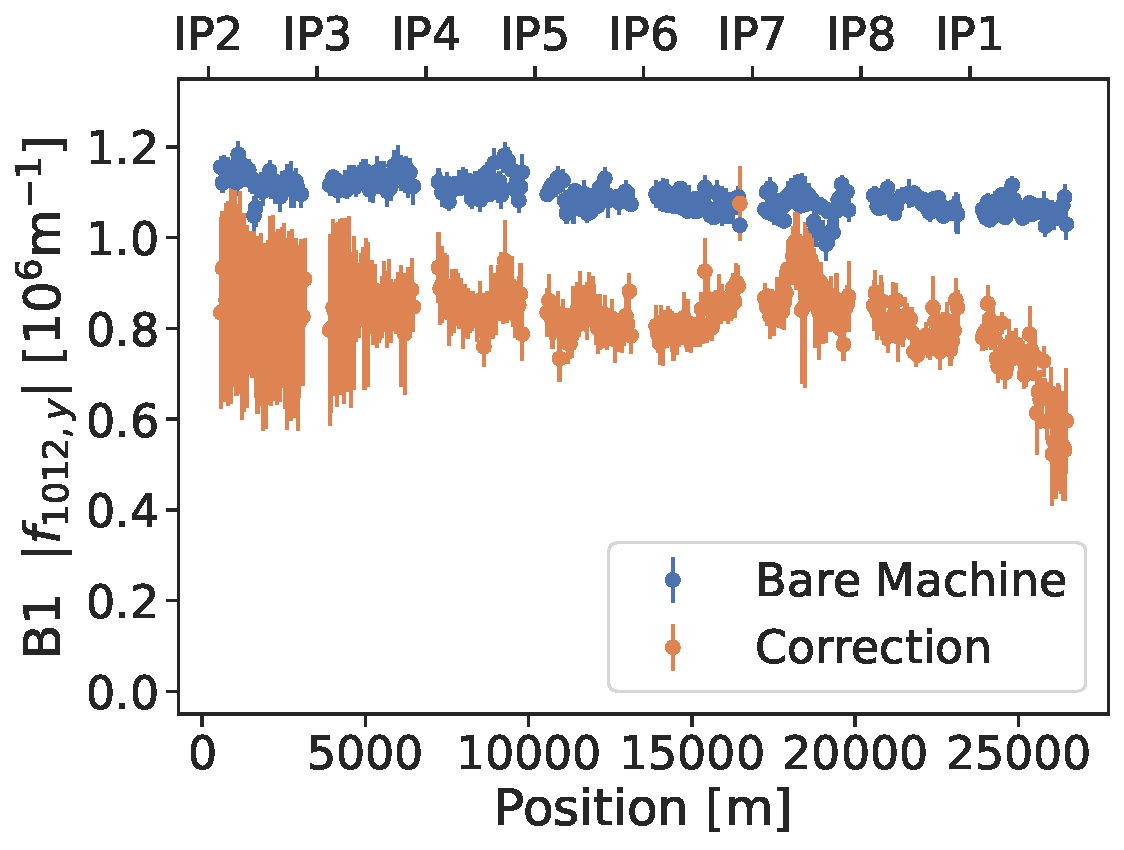
\includegraphics[width=\textwidth]{./images/f1012_b1.pdf}
        \caption{$f_{1012,y}$ Beam 1}
    \end{subfigure}
    \hfill
    \begin{subfigure}{0.49\textwidth}
        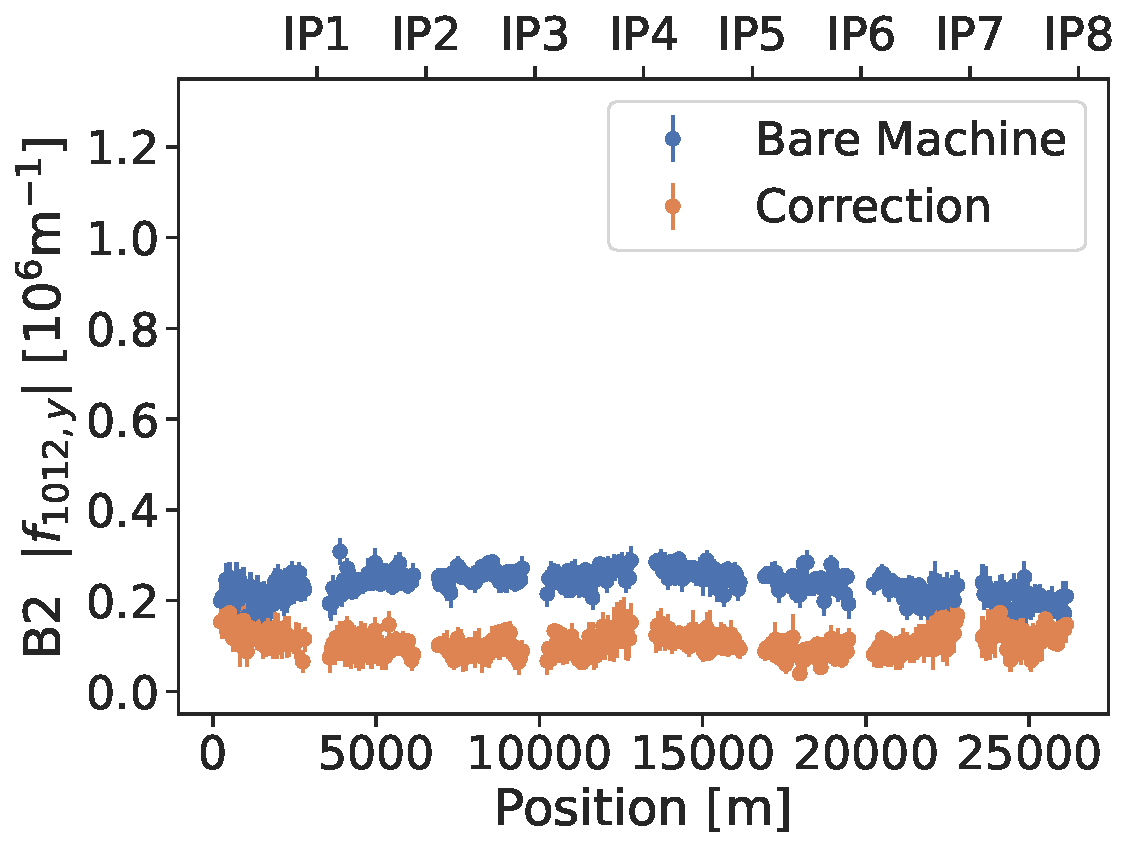
\includegraphics[width=\textwidth]{./images/f1012_b2.pdf}
        \caption{$f_{1012,y}$ Beam 2}
    \end{subfigure}
    %
    \par\bigskip 
    % 
    \begin{subfigure}{0.49\textwidth}
        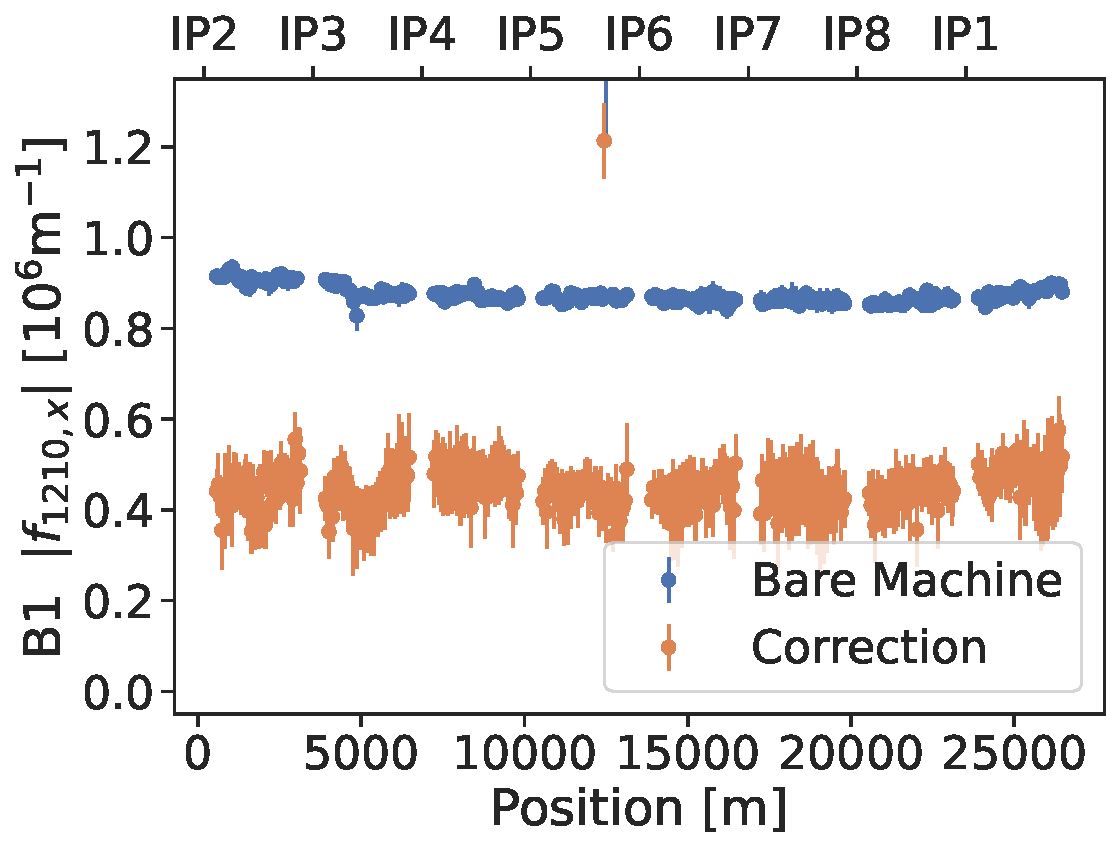
\includegraphics[width=\textwidth]{./images/f1210_b1.pdf}
        \caption{$f_{1210,x}$ Beam 1}
    \end{subfigure}
    \hfill
    \begin{subfigure}{0.49\textwidth}
        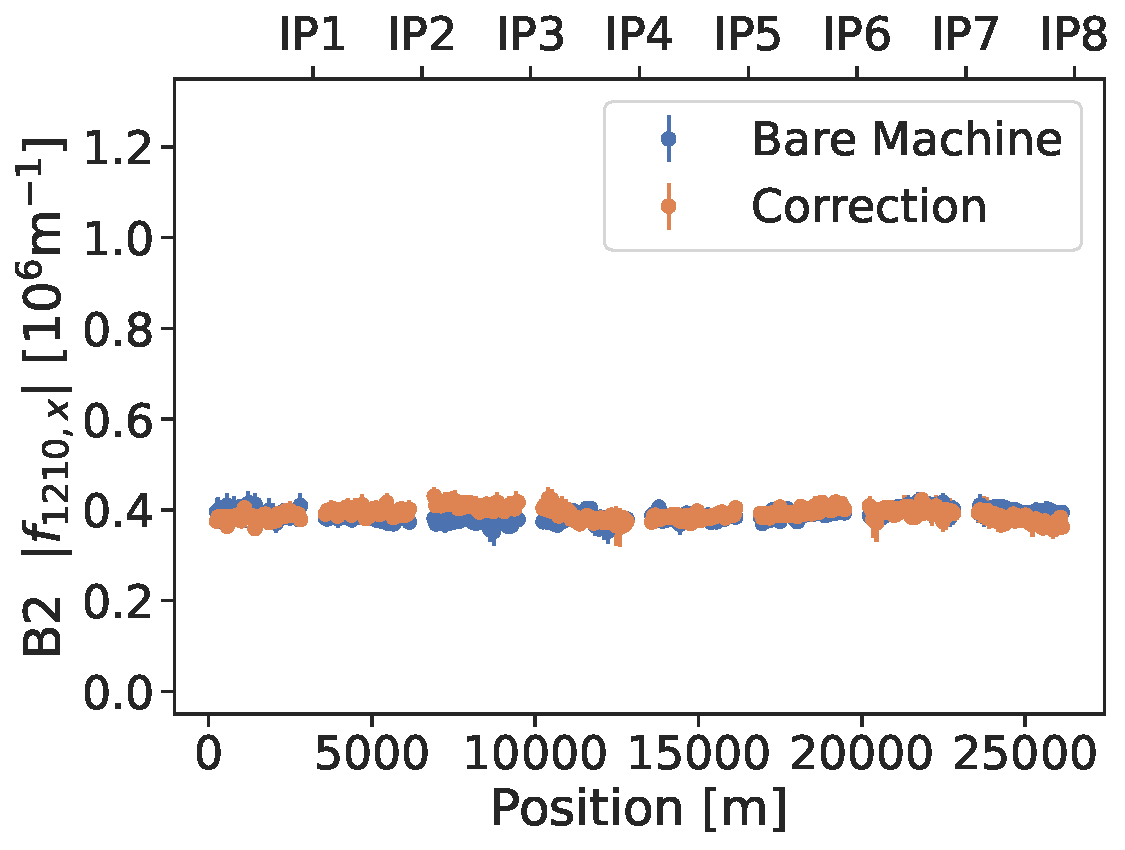
\includegraphics[width=\textwidth]{./images/f1210_b2.pdf}
        \caption{$f_{1210,x}$ Beam 2}
    \end{subfigure}
    \caption{Measured skew octupolar RDTs at top energy and $\beta^*=30\text{cm}$ before and after
    correction. A reduction if observed for all but one RDT in Beam 2.} 
    \label{fig:skew_octupolar:corrections_vs_bare}
\end{figure}






%=============================
%    Landau Contribution
%=============================
% https://indico.cern.ch/event/1351567/contributions/5708754/attachments/2773145/4832599/2023-12-15_MO_Roll_Coupling_complete.pdf
\FloatBarrier
\section{\review{Landau Octupoles Contribution}}


%-----------------------------
%        Introduction
%-----------------------------
\subsection{\review{Introduction}}

During the 2023 commissioning, measurements were taken at injection energy with different strengths
of Landau octupoles, where an unexpected shift in the skew octupolar RDTs was observed. Subsequent
measurements were conducted to better understand and characterize this contribution of normal
octupoles to skew octupolar fields. These new measurements were taken during an MD slot in September
2023 and focused on varying the strengths of the Landau octupoles to $-1K_4$, $\pm2 K_4$, $5K_4$.
All measurements were taken at injection energy at tunes of $Q_x = 0.275$, $Q_y = 0.293$ and
AC-Dipole deltas of $\Delta Q_x = -0.01$ and $\Delta Q_y = -0.011$. Although both beams were
measured, this section focuses on Beam 1 to preliminarily investigate the matter.  The following
\cref{fig:skew_octupolar:mo_different_levels_meas} illustrates the difference in amplitude of the
RDT $f_{1012}$ with these varying strengths.
\Cref{fig:skew_octupolar:mo_meas_vs_sim_+2} on the other hand shows the measured and simulated shift
of the same RDT from $0K_4$ to $+2K_4$. It is evident that simulations including normal and skew 
octupolar field errors are not enough to explain the behaviour observed in the measurements.

\begin{figure}[!htb]
    \centering
    \begin{subfigure}{0.8\textwidth}
        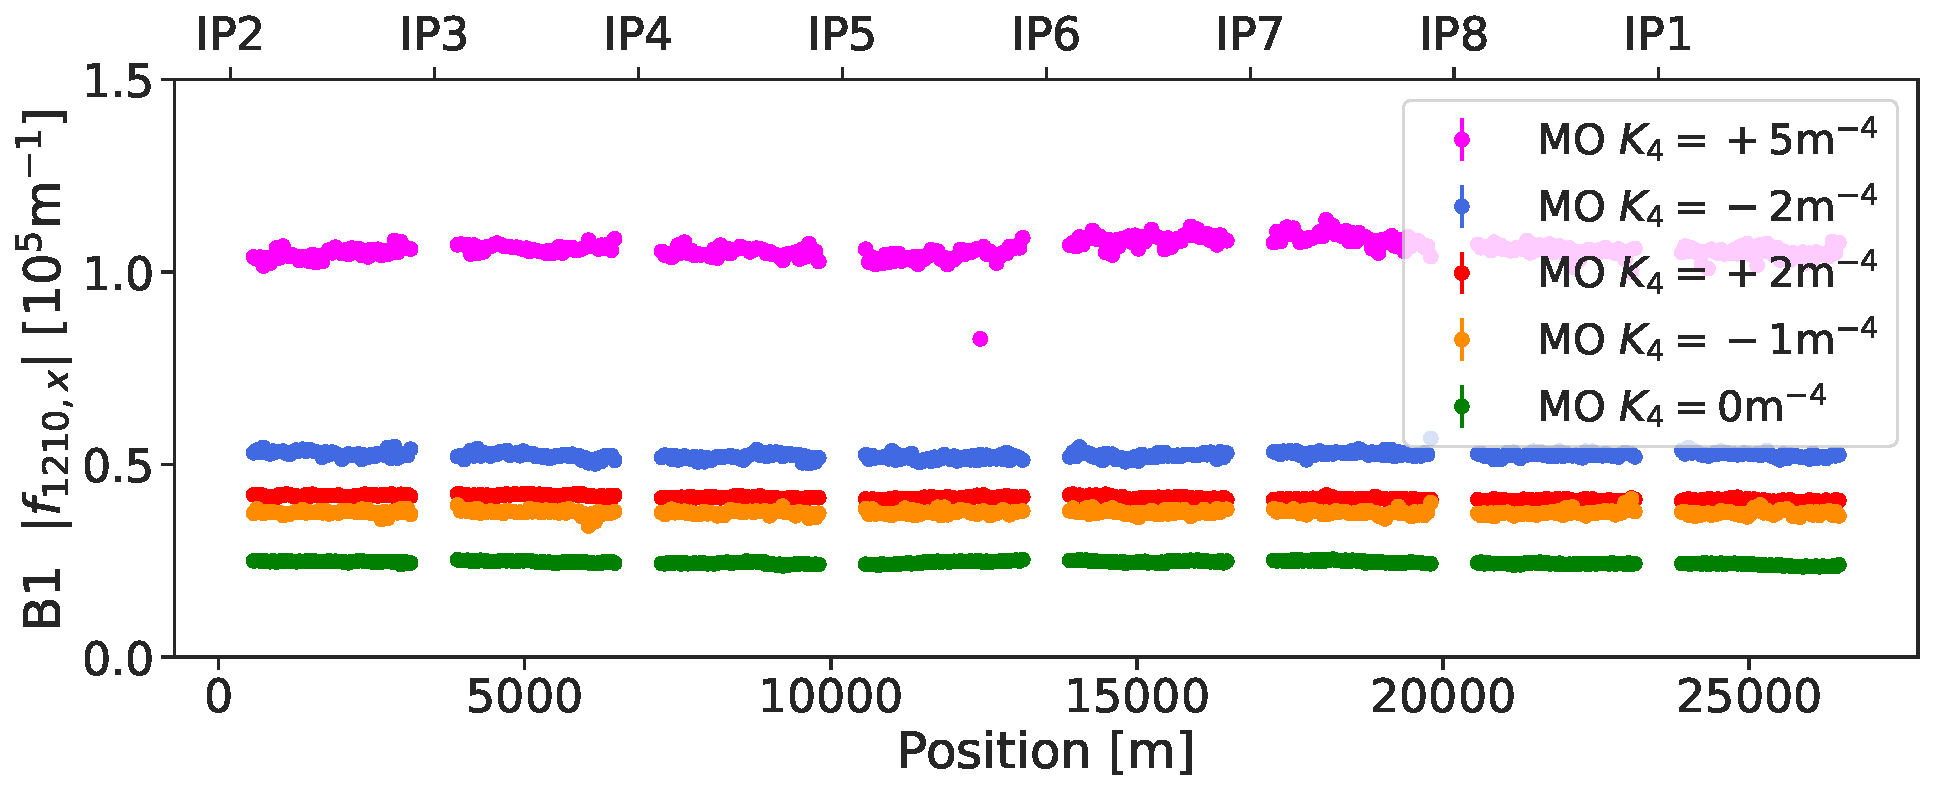
\includegraphics[width=\textwidth]{./images/skew_octupoles/f1210_AMP_all_measurements.pdf}
    \end{subfigure}
    \caption{Unexpected difference of skew octupolar RDT amplitudes with varying Landau octupoles
    strengths.}
    \label{fig:skew_octupolar:mo_different_levels_meas}
\end{figure}

\begin{figure}[!htb]
    \centering
    \begin{subfigure}{0.8\textwidth}
        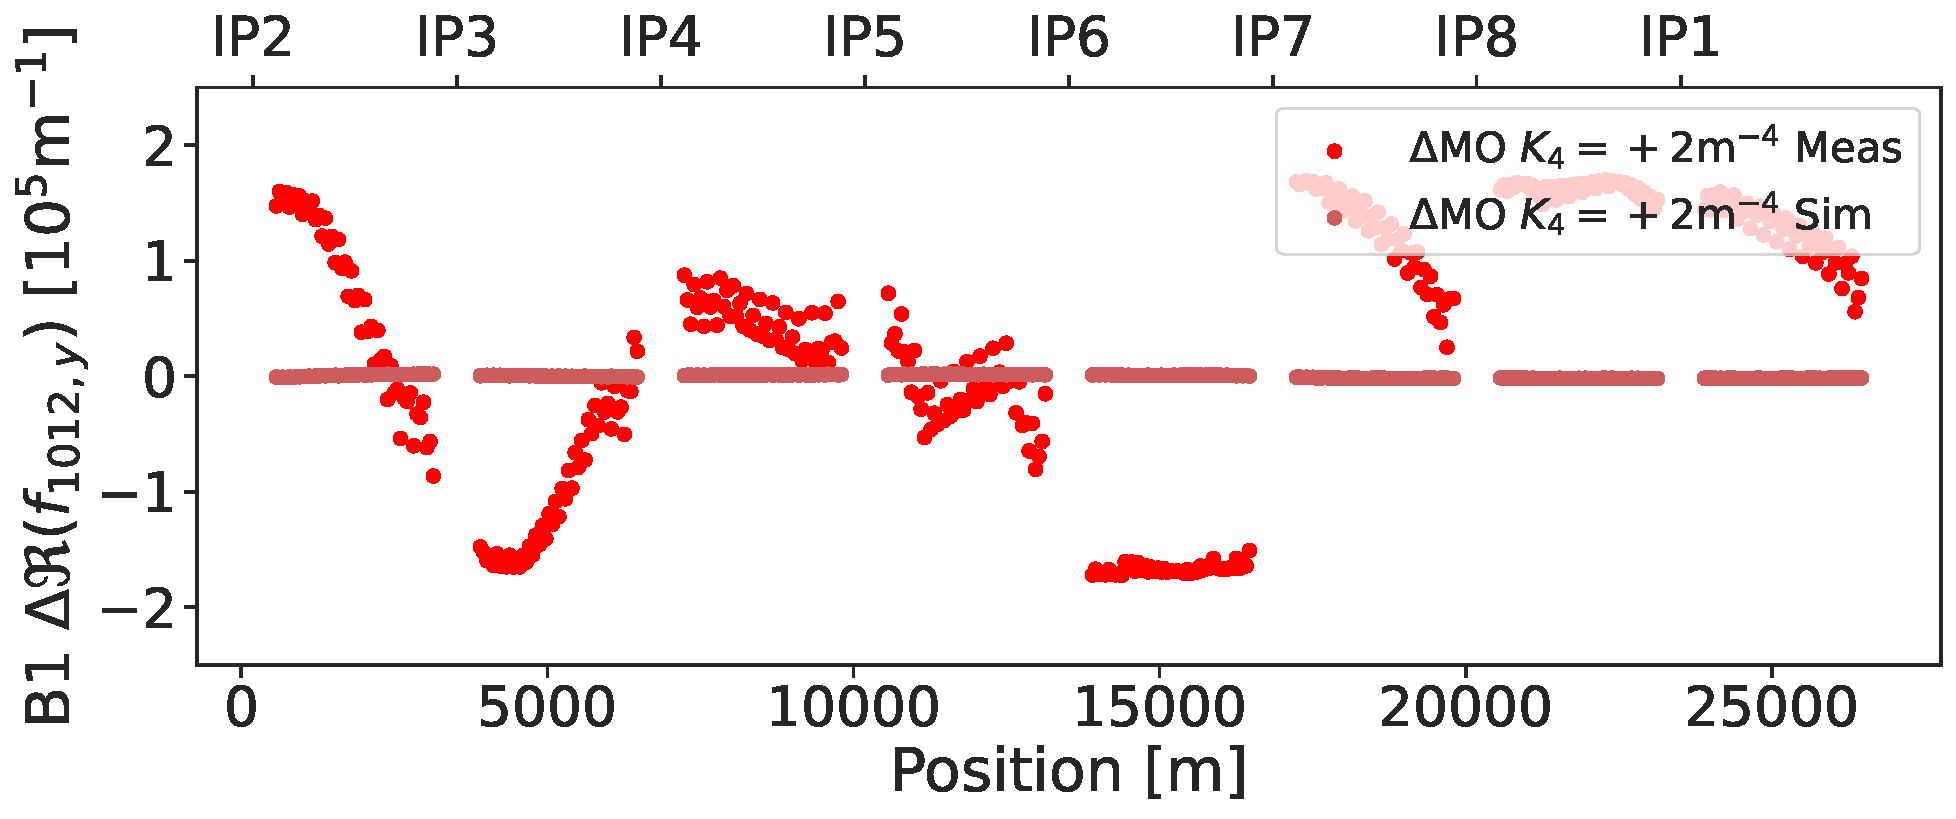
\includegraphics[width=\textwidth]{./images/skew_octupoles/f1012_meas_vs_sim_0shift.pdf}
        %\caption{$f_{1012,y}$}
    \end{subfigure}
    \caption{Measured and simulated shift of skew octupolar RDT after increase of Landau octupoles
    strength from zero. It is apparent that the shift in measurement is not replicated by the
    simulation.}
    \label{fig:skew_octupolar:mo_meas_vs_sim_+2}
\end{figure}



%-----------------------------
%        Misalignments
%-----------------------------
\subsection{\review{Misalignments}}

Magnet misalignments, more specifically roll errors, can generate skew magnetic fields instead of
the expected normal ones. To determine if this could explain the behaviour observed in measurements,
a tracking simulation was conducted with and without roll errors applied to the Landau octupoles.
The resulting RDTs reveal an imperceptible difference, unable to account for  the previously seen
shifts. The real part of the RDT $f_{1012}$ is shown in \cref{fig:skew_octupolar:sim_misalign},
with similar results seen in the other component and in $f_{1210}$.

\begin{figure}[!htb]
    \centering
    \begin{subfigure}{0.8\textwidth}
        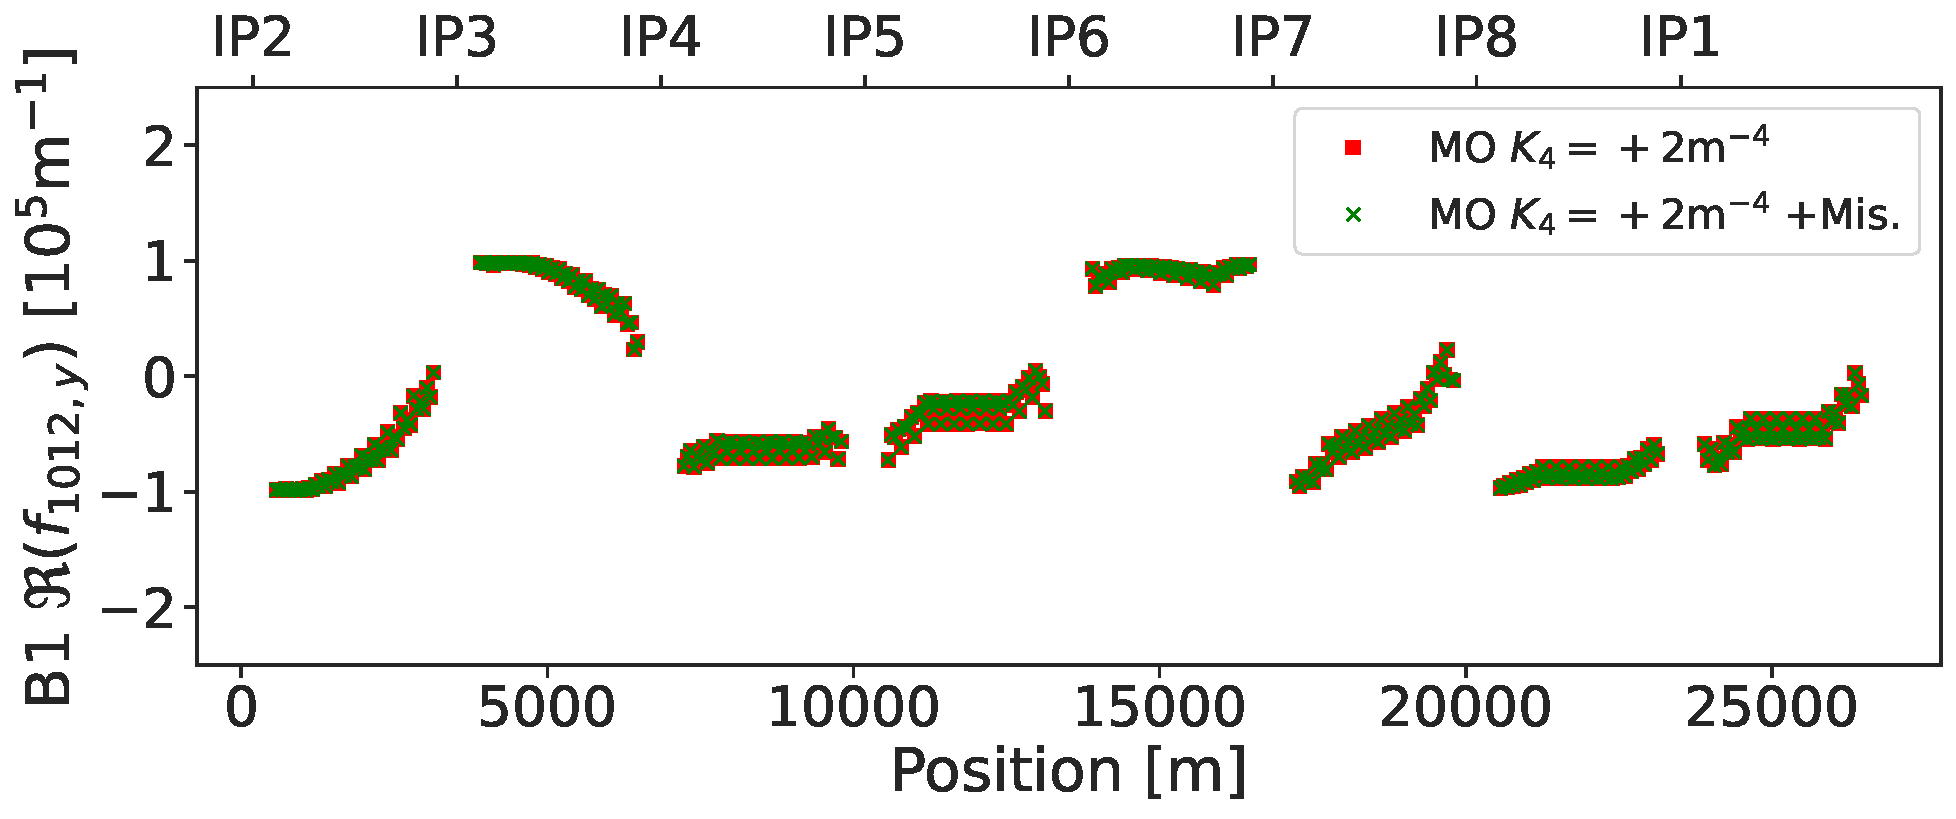
\includegraphics[width=\textwidth]{./images/skew_octupoles/f1012_misalign_REAL.pdf}
        %\caption{$f_{1012,y}$}
    \end{subfigure}
    \caption{Simulated skew octupolar RDT with normal and skew octupolar errors and Landau octupoles
    powered. One simulation includes further alignment errors on the Landau octupoles. No 
    significant difference is observed between the two.}
    \label{fig:skew_octupolar:sim_misalign}
\end{figure}



%-----------------------------
%        Coupling
%-----------------------------
\subsection{\review{Coupling}}

As misalignments could not explain the discrepancy, simulations were first run with varying values
of coupling at a fixed octupolar strength, allowing to gage the impact of coupling only.
\Cref{appendix:transfer_map:skew_quadrupole_and_octupole} details how coupling, in the form of a
skew quadrupole, combined with a normal octupole can generate skew quadrupolar-like fields.
The resulting RDT $f_{1012}$ is shown in \cref{fig:skew_octupolar:sim_coupling}, a similar trend is
observed for $f_{1210}$.
The presented $C^{-}$ values are commonly seen in operation and well below that of the
tolerances of the design of the LHC~\cite{bruning_lhc_2004}. As coupling increases, the skew
octupolar RDTs are expected to be significantly altered.

\begin{figure}[!htb]
    \centering
    \begin{subfigure}{0.8\textwidth}
        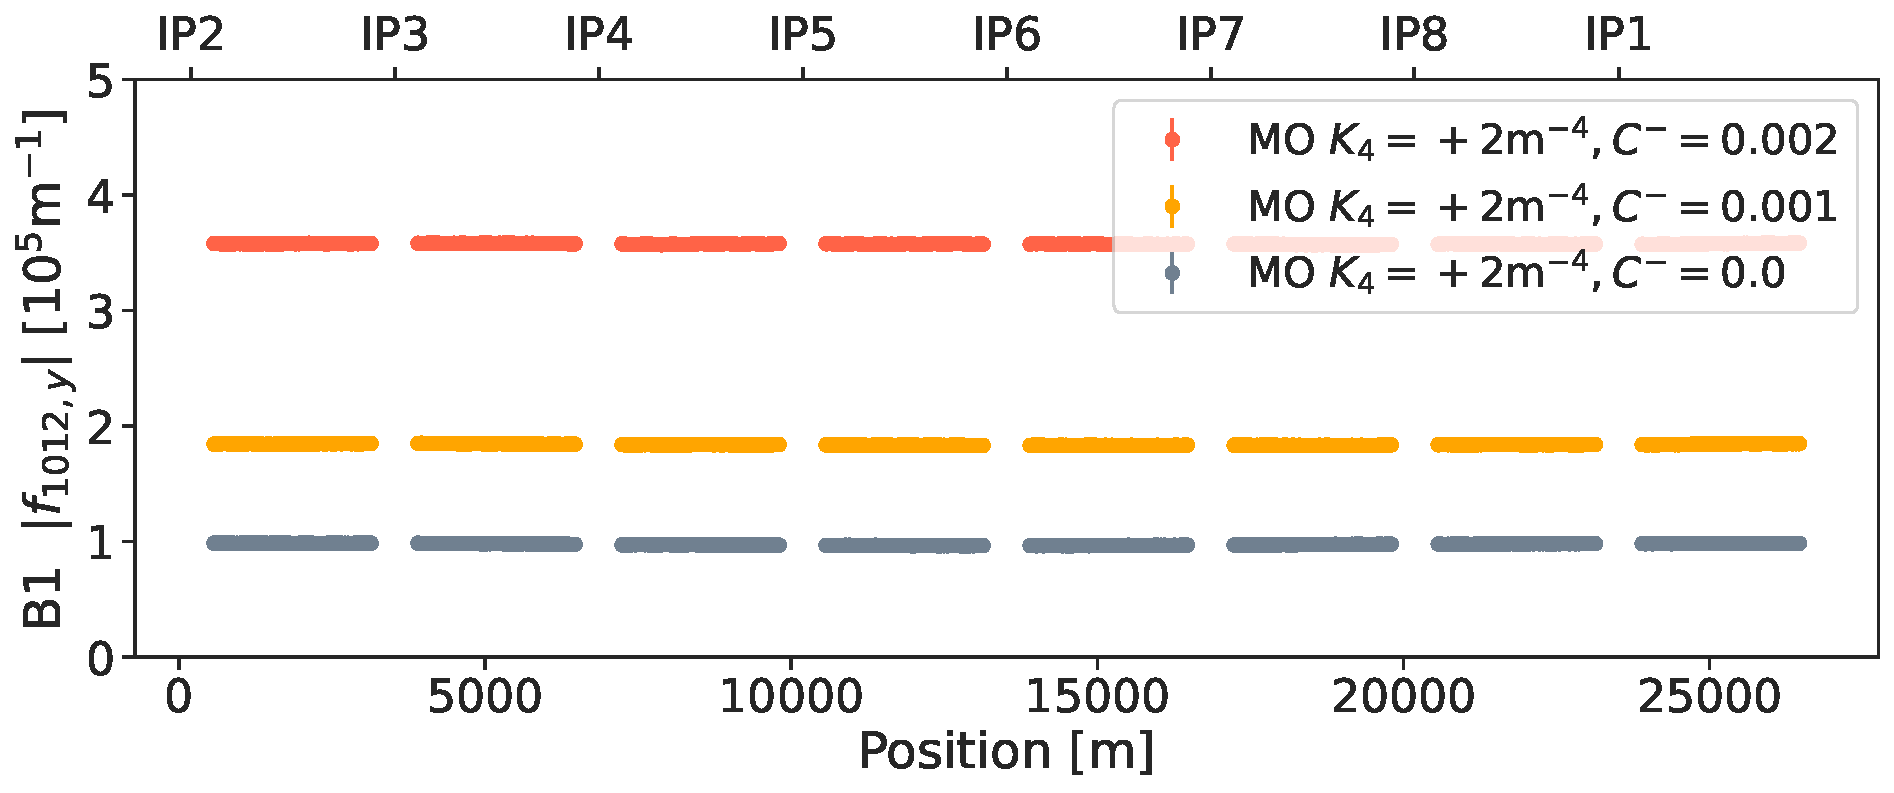
\includegraphics[width=\textwidth]{./images/skew_octupoles/f1012_coupling_sim_AMP.pdf}
        %\caption{$f_{1012,y}$}
    \end{subfigure}
    \caption{Simulated skew octupolar RDT with fixed Landau octupole strength but varying coupling.
    Selected coupling values are often seen in operation.}
    \label{fig:skew_octupolar:sim_coupling}
\end{figure}



%-----------------------------
%          Responses
\FloatBarrier
\subsubsection{\review{Responses with Coupling}}

\begin{wraptable}{r}{0.4\textwidth}
    \centering
    \begin{tabular}{cccc}
    \toprule
    &&\multicolumn{2}{c}{Rel. Diff. [\%]} \\
    \cmidrule{3-4}
    $K_4$ $[\text{m}^{-4}]$ & RDT & Real & Imag. \\
    \midrule
    \multirow{2}{*}{+5}
     & $f_{1210}$ & 12  & 10  \\
     & $f_{1012}$ & 17  & 16  \\[0.5em]
    \multirow{2}{*}{+2}
     & $f_{1210}$ & 12  & 13  \\
     & $f_{1012}$ & 15  & 16  \\[0.5em]
    \multirow{2}{*}{-1}
     & $f_{1210}$ & 117 & 119 \\
     & $f_{1012}$ & 132 & 133 \\[0.5em]
    \multirow{2}{*}{-2}
     & $f_{1210}$ & 50  & 50  \\
     & $f_{1012}$ & 123 & 120 \\
    \bottomrule
    \end{tabular}
    \caption{Relative difference between measured and simulated RDT shift induced by the
    Landau octupoles in presence of coupling. Real parts are illustrated in
    \cref{fig:skew_octupolar:response_meas_sim_coupling}.}
    \label{tab:skew_octupolar:rms_ratios}
\end{wraptable}

After recognizing that coupling could significantly contribute to the creation of skew
octupolar fields with normal octupoles, additional simulations were performed matching the measured
coupling for each set of measurements. The shift in real part of the RDTs $f_{1012}$ and $f_{1210}$
is shown in \cref{fig:skew_octupolar:response_meas_sim_coupling}, with a similar pattern observed
for the imaginary part. The relative RMS deviation between simulations and measurements is given
for each set of strengths and RDTs in \cref{tab:skew_octupolar:rms_ratios}.

It can be observed that simulations and measurements for positive strengths ($K_4=2$ and $K_4=5$) 
are now in good agreement. This suggests that the primary contribution to the skew octupolar RDTs
can be attributed to the Landau octupoles and coupling.
It is important to note that measurements with \textit{negative} strength show a response opposite
to what is predicted by simulations. This behaviour is not yet understood and requires further
investigation.

\begin{figure}[!htb]
    \centering
    \begin{subfigure}{0.47\textwidth}
        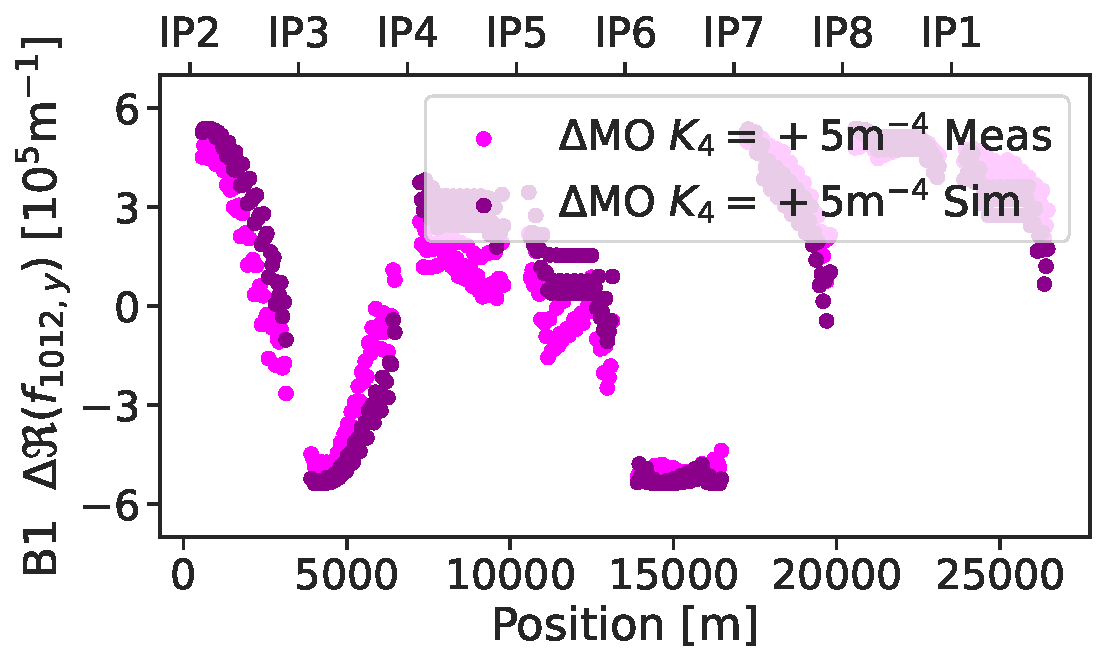
\includegraphics[width=\textwidth]{./images/skew_octupoles/responses_coupling/f1012_response_meas_sim_+5_REAL_smoll.pdf}
        %\caption{$f_{1012,y}$ for $K_4 = +5$}
    \end{subfigure}
    \hfill
    \begin{subfigure}{0.47\textwidth}
        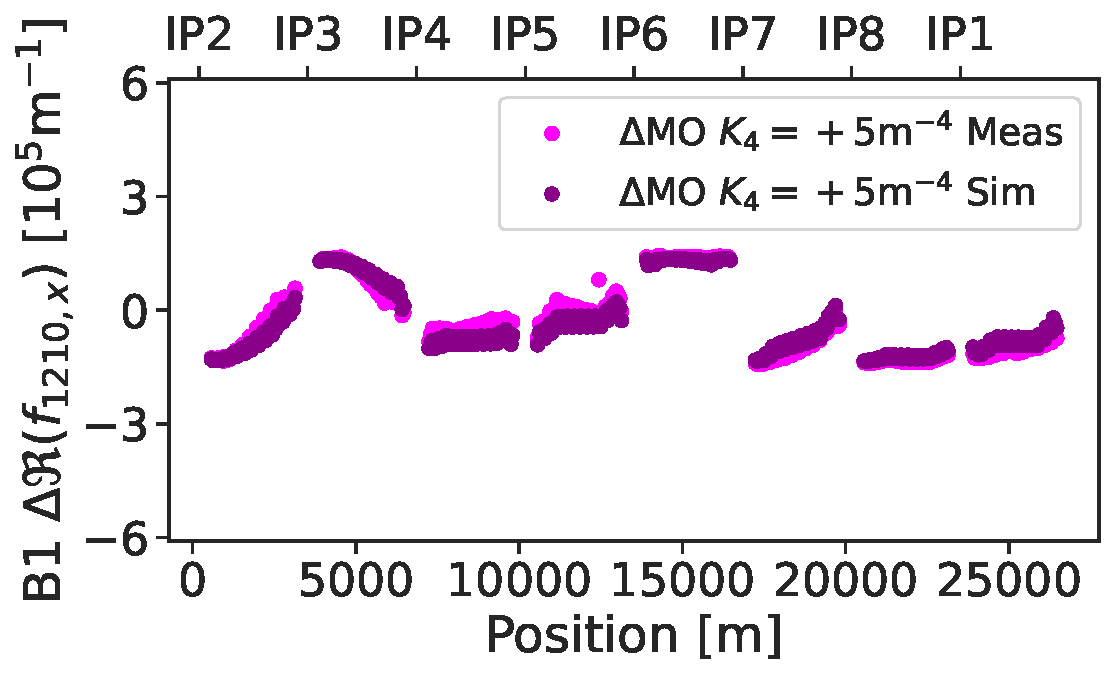
\includegraphics[width=\textwidth]{./images/skew_octupoles/responses_coupling/f1210_response_meas_sim_+5_REAL_smoll.pdf}
        %\caption{$f_{1210,x}$ for $K_4 = +5$}
    \end{subfigure}
    %
    \par\medskip 
    %
    \begin{subfigure}{0.47\textwidth}
        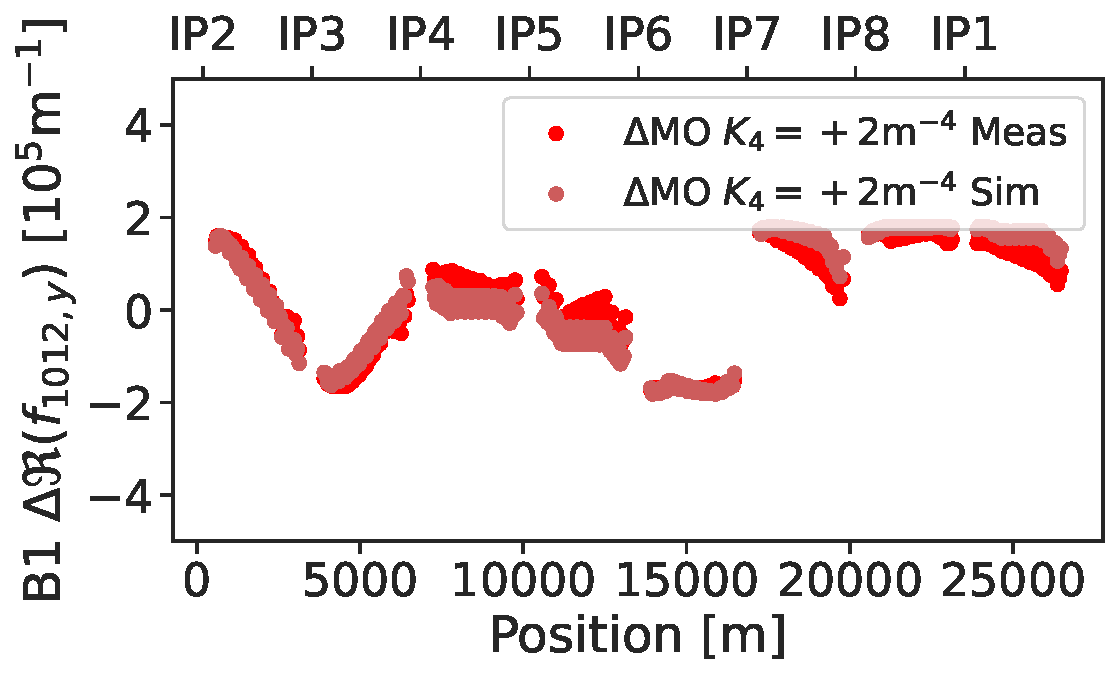
\includegraphics[width=\textwidth]{./images/skew_octupoles/responses_coupling/f1012_response_meas_sim_+2_REAL_smoll.pdf}
        %\caption{$f_{1012,y}$ for $K_4 = +2$}
    \end{subfigure}
    \hfill
    \begin{subfigure}{0.47\textwidth}
        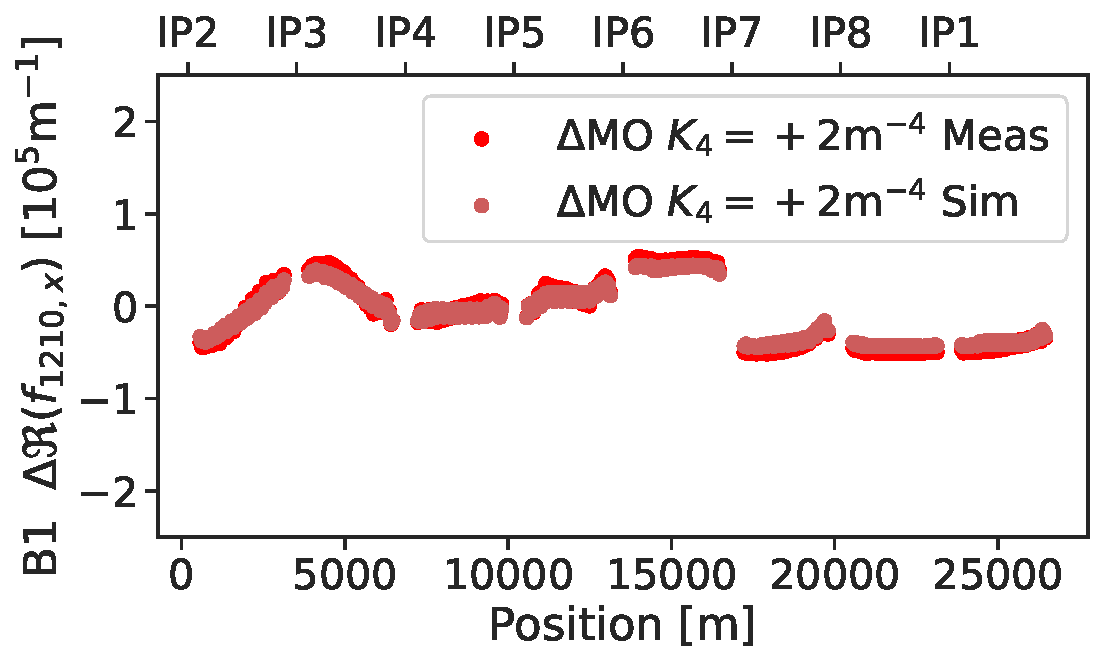
\includegraphics[width=\textwidth]{./images/skew_octupoles/responses_coupling/f1210_response_meas_sim_+2_REAL_smoll.pdf}
        %\caption{$f_{1210,x}$ for $K_4 = +2$}
    \end{subfigure}
    %
    \par\medskip 
    %
    \begin{subfigure}{0.47\textwidth}
        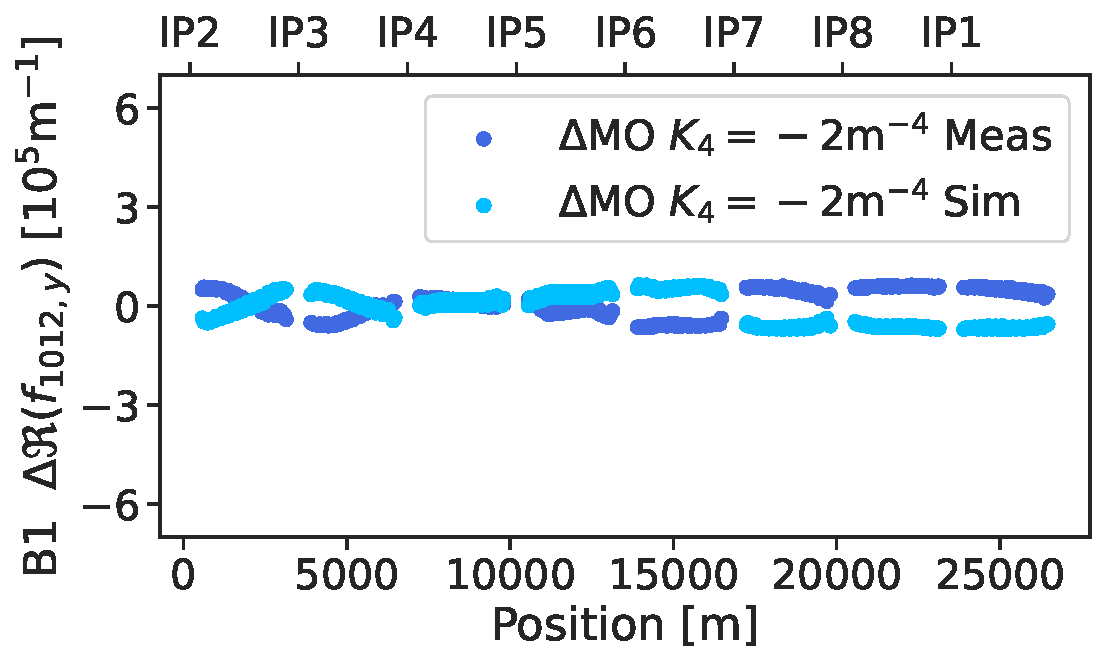
\includegraphics[width=\textwidth]{./images/skew_octupoles/responses_coupling/f1012_response_meas_sim_-2_REAL_smoll.pdf}
        %\caption{$f_{1012,y}$ for $K_4 = -2$}
    \end{subfigure}
    \hfill
    \begin{subfigure}{0.47\textwidth}
        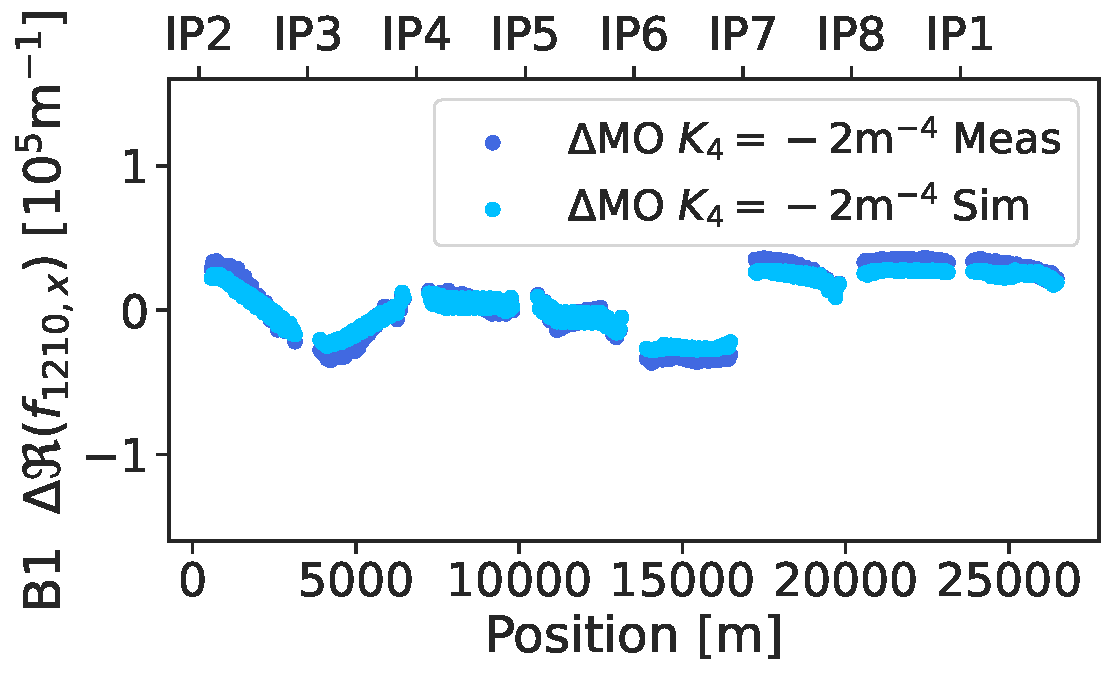
\includegraphics[width=\textwidth]{./images/skew_octupoles/responses_coupling/f1210_response_meas_sim_-2_REAL_smoll.pdf}
        %\caption{$f_{1210,x}$ for $K_4 = -2$}
    \end{subfigure}
    %
    \par\medskip 
    %
    \begin{subfigure}{0.47\textwidth}
        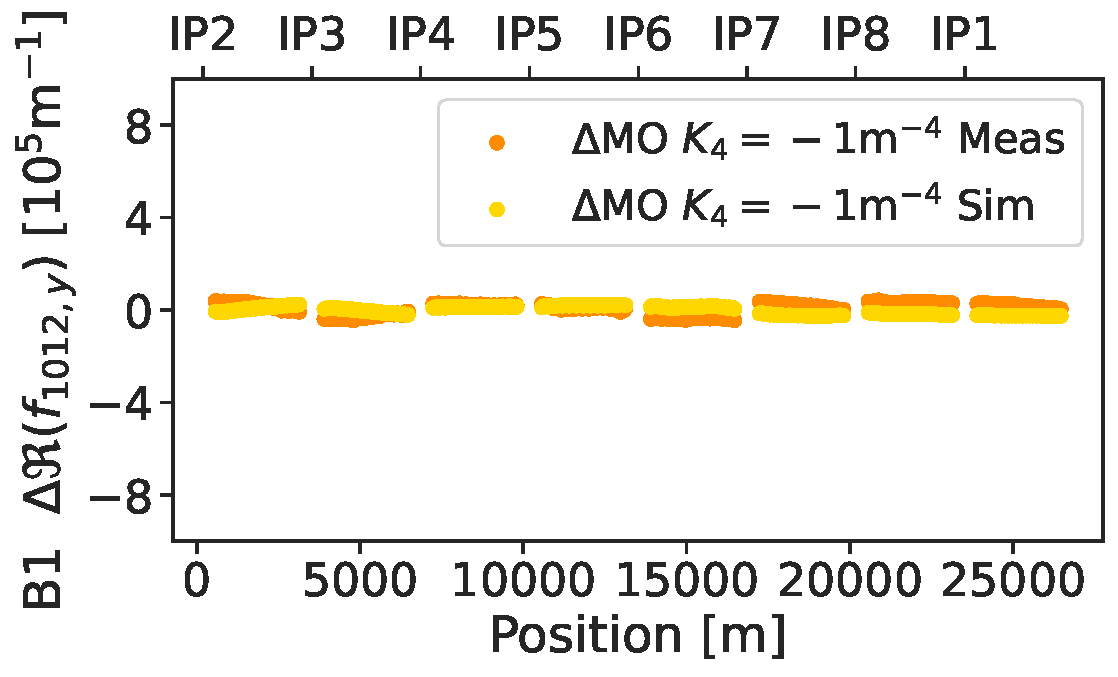
\includegraphics[width=\textwidth]{./images/skew_octupoles/responses_coupling/f1012_response_meas_sim_-1_REAL_smoll.pdf}
        %\caption{$f_{1012,y}$ for $K_4 = -1$}
    \end{subfigure}
    \hfill
    \begin{subfigure}{0.47\textwidth}
        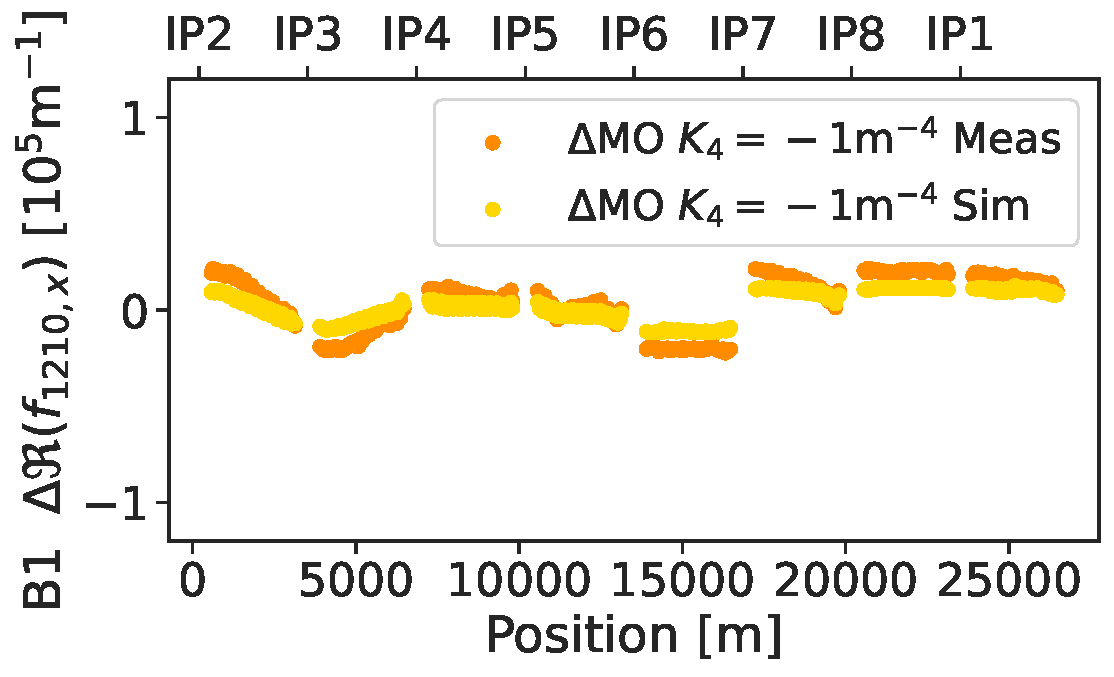
\includegraphics[width=\textwidth]{./images/skew_octupoles/responses_coupling/f1210_response_meas_sim_-1_REAL_smoll.pdf}
        %\caption{$f_{1210,x}$ for $K_4 = -1$}
    \end{subfigure}
    %
    \caption{Measured and simulated real part shift of skew octupolar RDTs induced by Landau
    octupoles in presence of coupling at injection energy. Left column shows $f_{1012}$ while right
    shows $f_{1210}$.}
    \label{fig:skew_octupolar:response_meas_sim_coupling}
\end{figure}





%=============================
%        Conclusion
%=============================
\FloatBarrier
\section{\todo{Summary}}